\documentclass[fontset=none]{article} %取消CTeX的默认字体设置

\usepackage[UTF8]{ctex}
\usepackage{fancyhdr}
\usepackage{extramarks}
\usepackage{amsmath}
\usepackage{amsthm}
\usepackage{tikz}
\usepackage[plain]{algorithm}
\usepackage{algpseudocode}
\usepackage{lmodern}
\usepackage{tikz}

% 处理
\usepackage[english]{babel}
\usepackage{hyperref}
\hypersetup{
    colorlinks=true,
    linkcolor=blue,
    filecolor=magenta,      
    urlcolor=cyan,
}

\newtheorem{theorem}{Theorem}

%
% Basic Document Settings
%
\setCJKmainfont{SourceHanSansCN-Light}



\topmargin=-0.45in
\evensidemargin=0in
\oddsidemargin=0in
\textwidth=6.5in
\textheight=9.0in
\headsep=0.25in

\linespread{1.1}

\pagestyle{fancy}
\lhead{\hmwkAuthorName}
\rhead{\firstxmark}
\lfoot{\lastxmark}
\cfoot{\thepage}

\renewcommand\headrulewidth{0.4pt}
\renewcommand\footrulewidth{0.4pt}

\setlength\parindent{0pt}

%
% Create Problem Sections
%

\newcommand{\enterProblemHeader}[1]{
    \nobreak\extramarks{}{Problem \arabic{#1} continued on next page\ldots}\nobreak{}
    \nobreak\extramarks{Problem \arabic{#1} (continued)}{Problem \arabic{#1} continued on next page\ldots}\nobreak{}
}

\newcommand{\exitProblemHeader}[1]{
    \nobreak\extramarks{Problem \arabic{#1} (continued)}{Problem \arabic{#1} continued on next page\ldots}\nobreak{}
    \stepcounter{#1}
    \nobreak\extramarks{Problem \arabic{#1}}{}\nobreak{}
}

\setcounter{secnumdepth}{0}
\newcounter{partCounter}
\newcounter{homeworkProblemCounter}
\setcounter{homeworkProblemCounter}{1}
\nobreak\extramarks{Problem \arabic{homeworkProblemCounter}}{}\nobreak{}

%
% Homework Problem Environment
%
% This environment takes an optional argument. When given, it will adjust the
% problem counter. This is useful for when the problems given for your
% assignment aren't sequential. See the last 3 problems of this template for an
% example.
%
\newenvironment{homeworkProblem}[1][-1]{
    \ifnum#1>0
        \setcounter{homeworkProblemCounter}{#1}
    \fi
    \section{Exercise \arabic{homeworkProblemCounter}}
    \setcounter{partCounter}{1}
    \enterProblemHeader{homeworkProblemCounter}
}{
    \exitProblemHeader{homeworkProblemCounter}
}

%
% Homework Details
%   - Title
%   - Due date
%   - Class
%   - Section/Time
%   - Instructor
%   - Author
%

\newcommand{\hmwkTitle}{作业二}
\newcommand{\hmwkDueDate}{2020.6.20}
\newcommand{\hmwkClass}{高级算法}
\newcommand{\hmwkClassInstructor}{Professor xia}
\newcommand{\hmwkAuthorName}{\textbf{xueshi hu}}

%
% Title Page
%

\title{
    \vspace{2in}
    \textmd{\textbf{\hmwkClass:\ \hmwkTitle}}\\
    \vspace{3in}
}

\author{\hmwkAuthorName}
\date{}

\renewcommand{\part}[1]{\textbf{\large Part \Alph{partCounter}}\stepcounter{partCounter}\\}

%
% Various Helper Commands
%

% Useful for algorithms
\newcommand{\alg}[1]{\textsc{\bfseries \footnotesize #1}}

% For derivatives
\newcommand{\deriv}[1]{\frac{\mathrm{d}}{\mathrm{d}x} (#1)}

% For partial derivatives
\newcommand{\pderiv}[2]{\frac{\partial}{\partial #1} (#2)}

% Integral dx
\newcommand{\dx}{\mathrm{d}x}

% Alias for the Solution section header
\newcommand{\solution}{\textbf{\large Solution}}

% Probability commands: Expectation, Variance, Covariance, Bias
\newcommand{\E}{\mathrm{E}}
\newcommand{\Var}{\mathrm{Var}}
\newcommand{\Cov}{\mathrm{Cov}}
\newcommand{\Bias}{\mathrm{Bias}}

\begin{document}
\maketitle
\pagebreak


\begin{homeworkProblem}
1.
\[
  S(x,y,w)=F(x,y,0)H(0,w) + F(x,y,1)H(1,w)
\]

当$x$,$y$,$w$中间只有一个为1的时候,结果分别为
\[
  b*c + (a+b)*d = ad + bc + bd
\]

\[
  b*c + (a+b)*d = ad + bc + bd
\]

\[
  a*d + b*(c+d) = ad + bc + bd
\]

当$x$,$y$,$w$中间只有一个为0的时候,结果分别为

\[
  b*d + (a+b)*(c +d) = ac + bc + ad  + 2bd
\]

\[
  b*d + (a+b)*(c +d) = ac + bc + ad  + 2bd
\]

\[
  (a+b)*c + (a+2b)*d = ac + bc + ad + 2bd
\]

全部为0的时候:
\[
  ac + bd
\]
全部为1的时候:
\[
  (a+b)d + (a+2d)(c+d)
\]
所以,$S=[ac+bd, ad+bc+bd, ac + bc + ad + 2bd, (a+b)d + (a+2d)(c+d)]$

2. 
\begin{figure}[h!]
  \begin{center}
    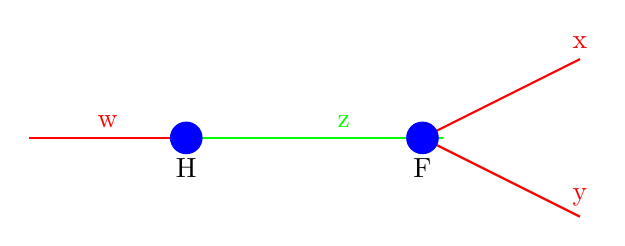
\begin{tikzpicture}
      \draw [red,thick] (-4,0) to (-2,0) -- node[above] {w} ++(-2,0) ;    

      \draw [red,thick] (1,0) to (3,1) -- node[above] {x} ++(0,0) ;    
      \draw [red,thick] (1,0) to (3,-1) -- node[above] {y} ++(0,0) ;    

      \draw [green,thick] (-2,0) to [out=0,in=0] (1,0) -- node[above] {z} ++(-2,0) ;    

      \draw [blue,fill] (-2,0) circle [radius=0.2] node [black,below=4] {H};
      \draw [blue,fill] (1,0) circle [radius=0.2] node [black,below=4] {F};
    \end{tikzpicture}
    \caption{函数为S的张量网络}
  \end{center}
\end{figure}

3. 在第一问中间计算,函数S的取值之和变量中间出现1的个数有关,而和其变量的取值分布无关,所以是
对称函数。

\end{homeworkProblem}

\begin{homeworkProblem}

当$H$节点数小于3的时候,可以多项式时间计算。下面分析这两种情况:
\begin{enumerate}    
  \item 当$H$的节点为1的时候,称之为$v$,$G$所有的节点只能映射到$v$,如果存在$v$到$v$的自环,那么存在唯一的映射,也就是所有的点映射到$v$。其实这种情况也是属于上课的时候分析过的rank=1的情况。

  \item 当$H$的节点为2的时候,$H$的两个节点为$u$,$v$,只需要分析导致$H$的rank=2的情况:
  \begin{enumerate}
    \item 没有自环,并且$u$$v$连通,求解映射可以转化为连通分量+环路检测判定问题。求解连通分量只需要简单的dfs或者bfs即可。检测其中是否存在环,只需要使用dfs就可以检查出来。
对于$G$中间的一个连通分量,如果可以全部映射一个节点,当其中没有环,将$G$构造为二分图,两个部分分别映射为一个节点。
    \item 存在两个,并且$u$$v$不连通,意味着在G中间原先存在边相连的点不能映射只能映射到相同的点上去,也就是说,$G$需要将整个连通分量映射到一个点,总的映射数量为$2^{N}$,其中N为G的连通分量的数量。
  \end{enumerate}
\end{enumerate}
综合上述,当$H$的节点数不大于3的时候,求解到$H$的同态数目是多项式时间可以求解的。
\end{homeworkProblem}

\end{document}
